\documentclass[journal]{IEEEtran}

\ifCLASSINFOpdf{}
\else
\usepackage[dvips]{graphicx}
\fi
\usepackage{url}
\usepackage{amsmath}
\hyphenation{op-tical net-works semi-conduc-tor}
\usepackage{hyperref}
\usepackage{graphicx}


\begin{document}

\title{SPCUP 2020: IEEE Signal Processing Cup 2020}

\author{Daniele Scapin, Gabriele Ferraresso, Marco Perin, Piero Simonetto, Riccardo Lorigiola
\thanks{This competition is sponsored by the IEEE Signal Processing Society and MathWorks}
\thanks{All author is with the University of Padue, Padova, ITA}}

\markboth{Journal of \LaTeX\ Class Files, March 2020}
{Shell \MakeLowercase{\textit{et al.}}: Bare Demo of IEEEtran.cls for IEEE Journals}
\maketitle

\begin{abstract}
In this letter, we proposed our method to solve the problem of unsupervised abnormality detection.
It involves four main steps: peaks and abnormalities during data acquisition saerch, anomaly check and system values update.

First and second steps take place at the same time during program flow but they serch autonomously the anomaly.
Peaks serch is implemented with the use of polyfit and Kalman evaluation, for prediction of the measures and 
alculation of the percentual change. Instead abnormalities during data acquisistion uses a modified version
of the isolation forest to verify if during the measures are occurred discrepancies.

The third part leverages of the concept that if every sensor in the autonomous system reports an anomaly, it means that
the behavior is not anomaly. The anomaly check uses a tree structure to get feedback from each sensor.

The system values update is used to improve respose time and to update the variables needed in other sections.
\end{abstract}

\begin{IEEEkeywords}
Abnormalities detection, peaks search, Kalman filter, isoaltion forest, tree structure
\end{IEEEkeywords}

\IEEEpeerreviewmaketitle{}

\section{Introduction}

\IEEEPARstart{}
{To do}
\\(Descrizione dettagliata flow del programma, associata al flow diagram)

\section{Peaks search: FindPeaksWrapper}

\(FindPeaksWrapper(\cdots)\) is used to find noticeable variation in the sensors data flow.
The program can be divided in four main elements: polyfit, Kalman filter, peak presence
and variables update.

\subsection{Polyfit}
For each sensor, for each new data acquisition the variation between the measure and the prediction
is checked by \(polyfit(\cdots)\) function (it uses \(polyfit(\cdots )\) and \(polyval(\cdots )\) Matlab functions).
This evaluation is done only if the number of elements to analyse is greater than degree of polyfit
evaluation plus three (in the program degree plus three). This restriction is caused by the necessity
of the presence of one element to verify and of degree plus two elements for \(polyfit(\cdots)\)
(plus two and not one because so the parametric estimation has al least a degree of freedom).

\subsection{Kalman Filter}
The Kalman filter is used only when the cosidered data is space, velocity and acceleration (angular or linear) and the acceleration is almost constant.
The Kalman filter needs the state transition matrix to be built (obtained from the differential equations of the model). In this case the model is a black box model thus it can't be described exactly. For these reasons the Kalman filter is used only on space, velocity and acceleration with uniform acceleration.
The Kalman filter is used anyway because if the autonomous system makes continuous and without variations paths/movements, it will generate a more accurate evaluation than \(polyfit\).
The filter is activated by the evaluation of slope of regression line (the coefficient is generated inside \(polyfit\) function).
The covariance matrix (\(Pn\_\cdots \)) is initialized as \(10\)\hspace{1mm}\(eye(\cdots)\) and update during subsequent cycles.
The covariance matrix of the measures (\(Q\)) is set by \(var2\_error\) vector placed diagonally (the motivation of these setting is explained in the next sections).

\subsection{Peaks Presence}
The peak presence is verified by calculating if the percentage of change between values expected and measured exceeds delta \([\%]\).
The value of delta is the maximum between a pre-set value (gap), the average percentage change of previous check and percentage error change of polyfit evaluation. This check is necessary because if signal noise is very loud, the function avoids reporting every measures as anomaly.

\subsection{Internal variables update}
Inside \(FindPeaksWrapper()\) there are three values (for each type of signal) that are used both as input and as output (\(Pn\_2, varp\_error, var2\_error\)) because in each cycle they are updated.
\(Pn\_2\) is necessary for Kalman filter evaluation and in each cycle it is updated whitin the function itself.
\(varp\_error\) is average percentage change between measure and prediction (error) (related to prediction).
\(var2\_error\) is average squared change between measure and prediction (error) and it is used in the covariance matrix of the measure.
It is used as covariance matrix of the measure because assuming the noises as gaussian noises (processes is subjected to ambient, thermal and internal noise)
\begin{displaymath}
    y_{measure} = y_{real} + e_{measure}  \quad  e_{measure}  \sim  N(0, \Sigma_{measure})
\end{displaymath}
\begin{displaymath}
    y_{estimate} = y_{real} + e_{estimate}  \quad  e_{estimate}  \sim  N(0, \Sigma_{estimate})
\end{displaymath}

The measures of different axis are considered unrelated (covariance matrix is diagonal).
Unidimensional estimation of variance
\begin{displaymath}
    e = y_{measure} - y_{estimate} \quad \quad \quad N(0, \theta)
\end{displaymath}
\begin{displaymath}
    e_{i} = y_{measure_{i}} - y_{estimate_{i}}
\end{displaymath}
\begin{displaymath}
    l_{e}(\theta) = -\log \left ( \prod_{i=1}^n p_{e_i}(\theta) \right ) 
\end{displaymath}
\begin{displaymath}
    \hspace{3mm} = \frac{n}{2}\log(2\pi) + \frac{n}{2}\log(\theta) + \sum_{i=1}^n \frac{e_i^2}{2\theta}
\end{displaymath}
\begin{displaymath}
    \frac{\partial l_{e}(\theta)}{\partial \theta} = \frac{n}{2\theta}- \sum_{i=1}^n \frac{e_i^2}{2\theta^2}
\end{displaymath}
\begin{displaymath}
    \hat\theta = \frac{\sum_{i=1}^n e_i^2}{n}
\end{displaymath}

\subsection{Input \- Output}
Detailed specification in \(FindPeaksWrapper(\cdots)\)
\\
\(Input\)
\begin{itemize}
\item t \(-\) time vector 
\item y \(-\) vector of values of data\_type element
\item data\_type \(-\) type of data
\item degree \(-\) max degree during poly fit evaluation
\item num \(-\) number of elements evaluating during polyfit
\item ap \(-\) maximum permissible percentage error
\item gap\_sva \(-\) max variation to identify a constant element
\end{itemize}

\(Output\)
\begin{itemize}
\item already\_analysed \(-\) true if all values of the corresponding data\_type are already analysed
\item anomaly \(-\) vector of all the anomaly of the corresponding data\_type
\item error \(-\) error of the last element (\(y_{measured}-y_{predicted}\))
\item y\_next \(-\) prediction of the last element
\end{itemize}


\section{Isolation Forest}
\(Isolation forest\) is a Statistical method to analyze small dataset and find anomalies. An anomaly is when an observation deviates so much from others.  In this case, anomalies are observation that not correspond to the right functioning of the Drone. We used this algorithm to analyze data when the observation received are approximately constant, we took this decision because we want to exclude the anomalies that could be find on the right functioning of the Drone. For example if we are height parameter we don’t add to isolation forest the observation of the drone when it’s  taking off, because there is a very high variation of the observation in a small time and this can be identified as a false positive anomaly. However, when the drone is flying, a high variation of the height in a small time is very likely an anomaly. 
This function can be divided in four main elements: \(Isolation Tree\), \(iForest\) and \(Anomalies Finder\)

\subsection{Isolation Tree}
This function randomly creates a binary tree from a given dataset of observation. It randomly take a subsample of the data. Our data are the observation and every observation can have one ore more dimension.
The function randomly select a dimension and a value in that dimension and divides observation in two groups (observation with a greater or equal value and observation with lower value). This process is recursively repeated until all observation are isolated. Isolated observation are on the leaves of the tree.

\begin{center}
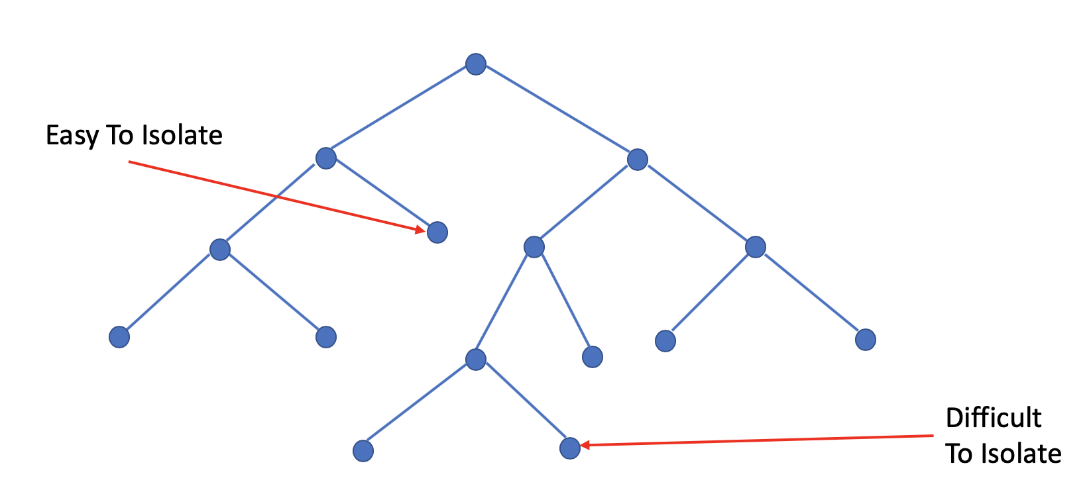
\includegraphics[width=\columnwidth]{albero.png}
\end{center}

\subsection{iForest}
This function creates a lot of different isolation trees that's why it’s called forest. Every tree is different because it’s randomly generated by \(IsolationTree\) function, however the observations inside every tree are always the same. \(iForest\) generate a forest that can be analyzed from \(Anomalies Finder\) function.

\subsection{Anomalies Finder}
This is the most important function of \(Isolation Forest\) because it’s used to find anomalies. It takes the forest and calculates the average height of every observation  and anomalies will have an average height lower than normal observations.

Now the anomaly score \(s\) of an instance \(x\) on a database of \(n\) instances is defined as:
\begin{gather*}
s(x,n)=2^ { \frac {{E(h(x))}} {c(n)} } \\
where \qquad c(n)=2H(n - 1) - \frac{n - 1}{n} \\
and \qquad H(i)=\ln (i) + 0.5772156649
\end{gather*}

\(s(x,n)\) give us an information about the observation:
\begin{itemize}
\item If \(s(x,n)\) is lower than \(0.5\), \(x\) is a normal value
\item If \(s(x,n)\) is closer to \(1\), \(x\) probably is an anomaly observation
\item If \(s(x,n)\) is around \(0.5\) for all observation it's safe to assume that the dataset doesn't contain anomalies.
\end{itemize}

\begin{center}
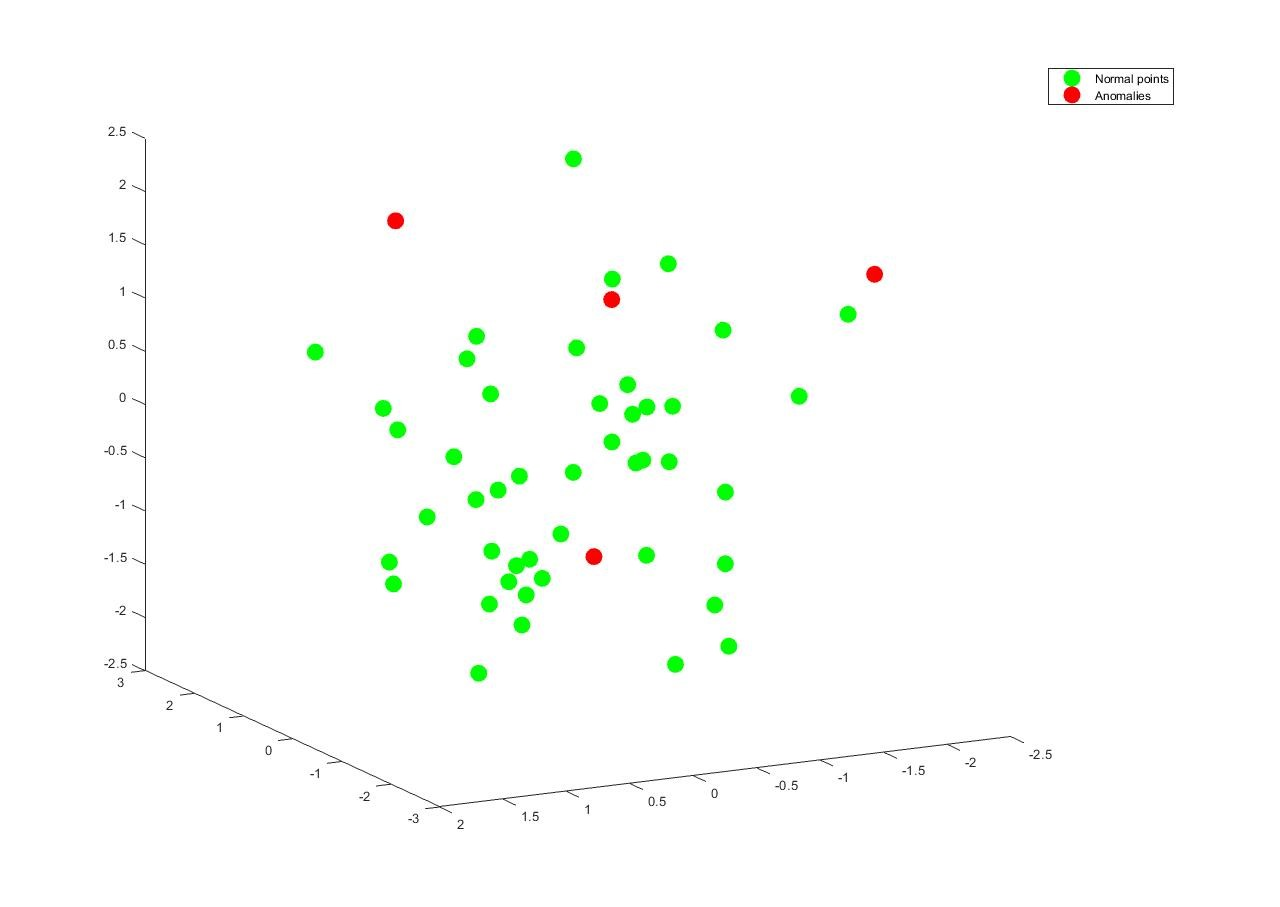
\includegraphics[width=\columnwidth]{grafico.jpg}
\end{center}

The main disadvantage of Isolation Forest is Swamping. Swamping is when normal instance are very closed to anomalies making them hard to be isolated. This problem can be minimized by subsampling the dataset.

\subsection{Input}
\begin{itemize}
\item NumTree: Number of trees inside the forest 
\item maxPoint: Maximum points inside every tree of the forest (for subsampling)
\item sk: Anomaly threshold 
\item type: Type of the new element 
\item newEl: New point of the forest 
\end{itemize}

\subsection{Output}

\begin{itemize}
\item Last: True if newEl is abnormal, false otherwise
\item Abnormal: True if there are abnormalities, False otherwise
\item posOfAnomaly: Index of abnormal points
\item h: Average height of each point in the forest
\item s: Anomaly score of each point in the forest
\end{itemize}


\begin{thebibliography}{References}
\bibitem{isolation forest 0}\href{https://cs.nju.edu.cn/zhouzh/zhouzh.files/publication/icdm08b.pdf?q=isolation-forest}{Isolation Forest.}

\bibitem{hariri forest} \href{http://www.ncsa.illinois.edu/Conferences/LSST18/assets/pdfs/hariri_forest.pdf}{Hariri Forest.}

\bibitem{isolation forest1} \href{https://medium.com/walmartlabs/swamping-and-masking-in-anomaly-detection-how-subsampling-in-isolation-forests-helps-mitigate-bb192a8f8dd5}{Swamping and masking in anomaly detection in isolation forest.}

\bibitem{isolation forest 2} \href{https://scikit-learn.org/stable/modules/generated/sklearn.ensemble.IsolationForest.html}{Anomaly score of isolation forest.}

\bibitem{isolation forest 3} \href{https://towardsdatascience.com/anomaly-detection-with-isolation-forest-visualization-23cd75c281e2}{Anomaly detection with isolation forest visualization.}

\end{thebibliography}


\section{Anomaly Check}
 
This part contains classes and functions to structure data in a prioritized way, 
to avoid unnecessary controls over sensor that are less likely to give data representing a true anomaly

\section{System Values Update}
The intantion is to build a real time program. To do this, the Bag manager has to adjust the reading time interval based on the time needed for the previous cicle.
For this reason, keeping the time of a balanced cicle is extremely crucial, so that t he function \(OptimizeParameter()\)
keeps track of it and set the parameter of the various components based on the previous values and the variation of time that it's involved in all the program.
The main idea is that if the program is fast enough, the algorithms can be even more precise otherwise they can be relaxed a bit.

\end{document}
